%%%%%%%%%%%%%%%%%%%%%%%%%%%%%%%%%%%%%%%%%%%%%%%%%%%%%%%%%%%%%%%%%%%%%%%%%%%%%%%%
%%%%%%%%%%%%%%%%%%%%%%%%%%%%%%%%%%%%%%%%%%%%%%%%%%%%%%%%%%%%%%%%%%%%%%%%%%%%%%%%
%%%%%%%%%%%%%%%%%%%%%%%%%%%%%%%%%%%%%%%%%%%%%%%%%%%%%%%%%%%%%%%%%%%%%%%%%%%%%%%%

\documentclass[a0,portrait]{a0poster}

% control margins here
\usepackage{geometry}
 \geometry{
 a0paper,
 left = 5cm,
 top = 4.5cm,
 right = 5cm,
 bottom = 2cm     %4.5cm
 }
\addtolength{\textwidth}{4.5cm} % width of text can be adjusted if margins above are adjusted

\usepackage{multicol} % This is so we can have multiple columns of text side-by-side
\columnsep=3em % This is the amount of white space between the columns in the poster
\columnseprule=0pt % This is the thickness of the black line between the columns in the poster

% UZH colours %%%%%%%%%%%%%%%%%%%%%%%%%%%%%%%%%%%%%%%%%%%%%%%%%%%%%%%%%%%%%%%%%%
%%%%%%%%%%%%%%%%%%%%%%%%%%%%%%%%%%%%%%%%%%%%%%%%%%%%%%%%%%%%%%%%%%%%%%%%%%%%%%%%
\usepackage[svgnames]{xcolor}
\definecolor{uzhblau100}{RGB}{0, 40, 165}
\definecolor{uzhblau80}{RGB}{51,83,183}
\definecolor{uzhockerrot100}{RGB}{220, 96, 39}
\definecolor{uzhockerrot80}{RGB}{227, 128, 82}
\definecolor{uzhflaschengruen100}{RGB}{42, 127, 98}
\definecolor{uzhflaschengruen80}{RGB}{86, 157, 133}
\definecolor{conclusion}{RGB}{204,212,237} % the conclusion box colour

% Packages %%%%%%%%%%%%%%%%%%%%%%%%%%%%%%%%%%%%%%%%%%%%%%%%%%%%%%%%%%%%%%%%%%%%%
%%%%%%%%%%%%%%%%%%%%%%%%%%%%%%%%%%%%%%%%%%%%%%%%%%%%%%%%%%%%%%%%%%%%%%%%%%%%%%%%

\usepackage{ifthen} % needed to stop horizontal line above 'Conclusions' section
\usepackage{graphicx} % Required for including images
\graphicspath{{figures/}} % Location of the graphics files
\usepackage{mwe,tikz}\usepackage[percent]{overpic} % overlay your photo over the background
\usepackage{booktabs} % Top and bottom rules for table
\usepackage[font=small,labelfont=bf]{caption} % Required for specifying captions to tables and figures
\usepackage{amsfonts, amsmath, amsthm, amssymb} % For math fonts, symbols and environments
\usepackage{wrapfig} % Allows wrapping text around tables and figures

\usepackage{fontspec} % custom fonts
\defaultfontfeatures[Palatino]
{
    Extension = .ttf,
    UprightFont = font/LT_41167,
    BoldFont = font/LT_41169,
    ItalicFont  = font/LT_41168,
    BoldItalicFont = font/LT_41170,
}
\defaultfontfeatures[TheSans]
{
    Extension = .otf,
    UprightFont = font/TheSans-LP5Plain,
    BoldFont = font/TheSans-LP7Bld,
    ItalicFont  = font/TheSans-LP5PlainIT,
    BoldItalicFont = font/TheSans-LP7BldIT,
}
\setmainfont{TheSans} % choose your font here
\usepackage[onehalfspacing]{setspace} % remove for single spacing
\usepackage{tcolorbox} % for the conclusions box
\usepackage{blindtext} % you can remove this once you add your content
\usepackage[export]{adjustbox} % allow floating a graphic right
\usepackage{titlesec} % customising section titles
\usepackage{needspace} % prevent break between line and section title
\usepackage{nameref} % package and command to get the name of the current section (for ifthen)
\usepackage{hyperref} % Hyperlinks
\usepackage{pifont} % More styles for bullets

% Start of the poster %%%%%%%%%%%%%%%%%%%%%%%%%%%%%%%%%%%%%%%%%%%%%%%%%%%%%%%%%%
%%%%%%%%%%%%%%%%%%%%%%%%%%%%%%%%%%%%%%%%%%%%%%%%%%%%%%%%%%%%%%%%%%%%%%%%%%%%%%%%
%%%%%%%%%%%%%%%%%%%%%%%%%%%%%%%%%%%%%%%%%%%%%%%%%%%%%%%%%%%%%%%%%%%%%%%%%%%%%%%%
\begin{document}

% define how our section titles will look (with ruled line)
\titleformat{\section}
  {\needspace{1\baselineskip}\sectionrule\huge\bfseries}
  {\color{uzhblau100}\thesection.}
  {1em}
  {\color{uzhblau100}}

\titleformat{\subsection}
  {\Large\bfseries}
  {\color{uzhblau100}}
  {0em}
  {\color{uzhblau100}}

% Draw a horizontal line before the section unless it is conclusions (if you change the name of Conclusions, you should also change it here too so it is recognised and the line suppressed
\makeatletter
\newcommand{\sectionrule}{%
 \ifthenelse{\equal{\@currentlabelname}{Conclusions}}
 % use the below line instead of the above if conclusions is a section*
 % \ifthenelse{\equal{\@currentlabelname}{}}
  {}
  {\vspace*{-\baselineskip}
   \vrule height 1pt depth 1pt width \linewidth\vskip0.4pt
   \bigskip}%
}
\makeatother

%%%%%%%%%%%%%%%%%%%%%%%%%%%%%%%%%%%%%%%%%%%%%%%%%%%%%%%%%%%%%%%%%%%%%%%%%%%%%%%%
% POSTER HEADER %%%%%%%%%%%%%%%%%%%%%%%%%%%%%%%%%%%%%%%%%%%%%%%%%%%%%%%%%%%%%%%%

% Title %%%%%%%%%%%%%%%%%%%%%%%%%%%%%%%%%%%%%%%%%%%%%%%%%%%%%%%%%%%%%%%%%%%%%%%%
\title{Anonymization of data for open science in psychology}

% Top logo %%%%%%%%%%%%%%%%%%%%%%%%%%%%%%%%%%%%%%%%%%%%%%%%%%%%%%%%%%%%%%%%%%%%%
\noindent
\begin{figure}[h]
\begin{minipage}{.15\linewidth}
  
\includegraphics[width=10cm]{Poster TEX/style/UZH.jpg} 
\end{minipage}
\begin{minipage}{.15\linewidth}
  
\includegraphics[width=10cm]{Poster TEX/style/FHNW.png} 
\end{minipage}
\begin{minipage}{.15\linewidth}
  
\includegraphics[width=10cm]{Poster TEX/style/SwissAnon.jpg} 
\end{minipage}
\hspace{\fill} % This will push the fourth image to the right
\begin{minipage}{.24\linewidth}
  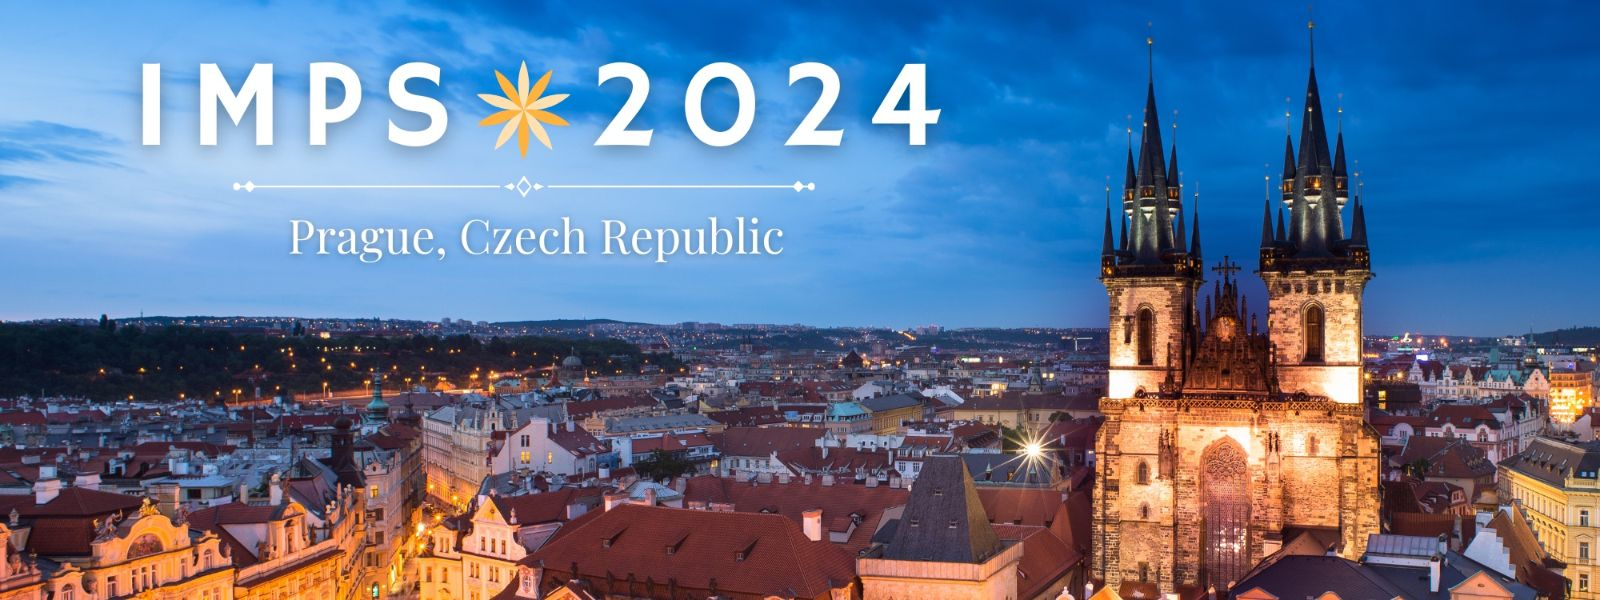
\includegraphics[width=20cm]{Poster TEX/style/IMPS.png}
\end{minipage}
\end{figure}

% Header formatting %%%%%%%%%%%%%%%%%%%%%%%%%%%%%%%%%%%%%%%%%%%%%%%%%%%%%%%%%%%%
% The header is divided into two boxes, on the left is the text and on the right is the image
\begin{minipage}[b][][t]{.6\linewidth}
\vfill
\makeatletter
\raggedright{\fontsize{92pt}{100pt}\selectfont\color{uzhblau100}\textbf{{\@title}}\par}
\makeatother
\color{Black}
\vspace{1cm}

% Subtitle %%%%%%%%%%%%%%%%%%%%%%%%%%%%%%%%%%%%%%%%%%%%%%%%%%%%%%%%%%%%%%%%%%%%%
%\Huge\textit{Subtitle goes here}\\[2.4cm] % Subtitle if it exists

% Author(s) %%%%%%%%%%%%%%%%%%%%%%%%%%%%%%%%%%%%%%%%%%%%%%%%%%%%%%%%%%%%%%%%%%%%
\underline{Jiří Novák\textsuperscript{1,2,3}} \\
\vspace{0.2cm}
\textsuperscript{1} University of Zürich, Psychological Methods, Evaluation and Statistics \\
\textsuperscript{2} University of Applied Sciences and Arts Northwestern Switzerland, Institute for Competitiveness and Communication \\
\textsuperscript{3} Swiss Data Anonymization Competence Center
%\texttt{you@uzh.ch}%\\ % add your email
\end{minipage}
%
\begin{minipage}[b][][t]{0.388\linewidth}
\vfill
  \begin{overpic}[width=.8\textwidth,right]{LIRI_WissPoster_Wasserzeichen.png
  } % what even is this thing?
     \put(85,0){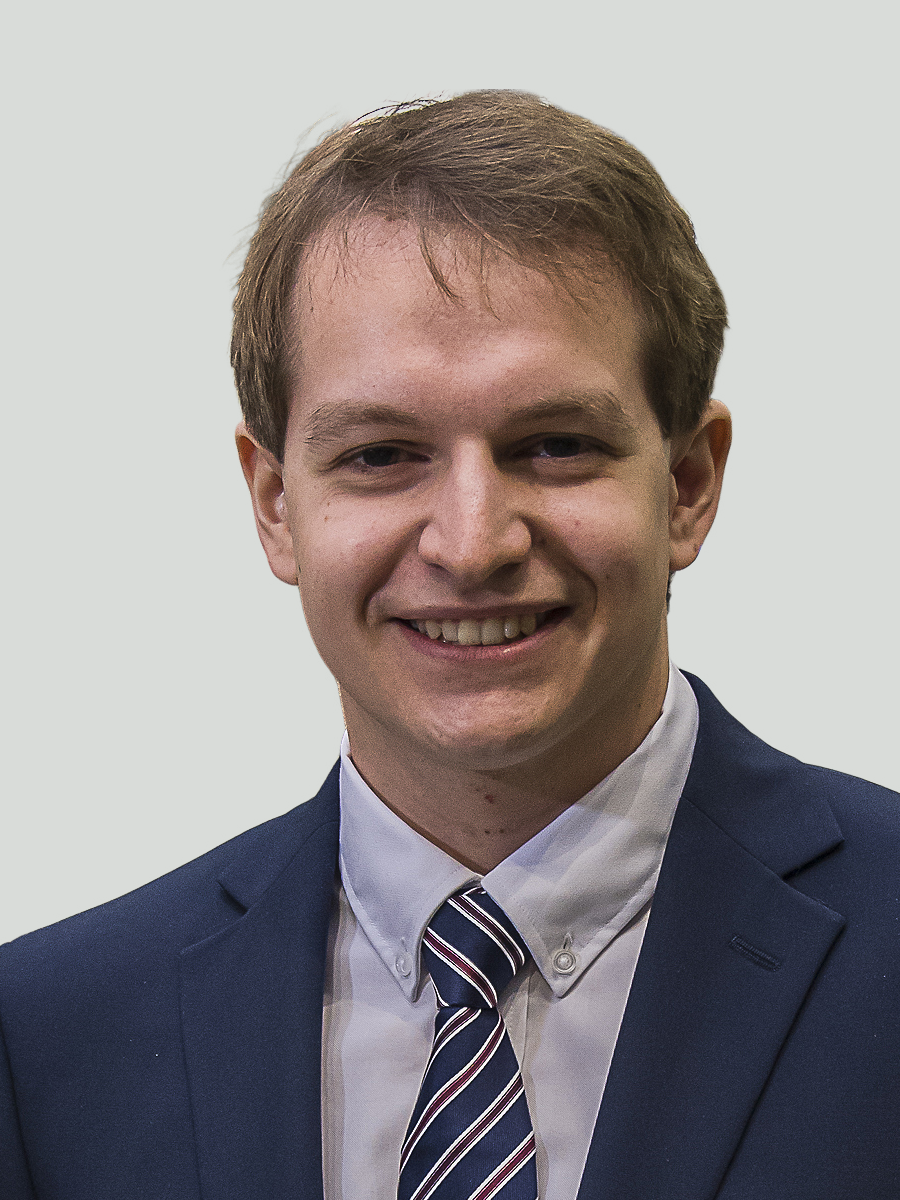
\includegraphics[scale=0.25]{Poster TEX/style/JN.png}}  % your image goes in here
  \end{overpic}
\end{minipage}
\vspace{1cm}

%%%%%%%%%%%%%%%%%%%%%%%%%%%%%%%%%%%%%%%%%%%%%%%%%%%%%%%%%%%%%%%%%%%%%%%%%%%%%%%%
%%%%%%%%%%%%%%%%%%%%%%%%%%%%%%%%%%%%%%%%%%%%%%%%%%%%%%%%%%%%%%%%%%%%%%%%%%%%%%%%
% POSTER BODY %%%%%%%%%%%%%%%%%%%%%%%%%%%%%%%%%%%%%%%%%%%%%%%%%%%%%%%%%%%%%%%%%%
\begin{multicols}{3} % This is how many columns your poster will be broken into

\Large
%%%%%%%%%%%%%%%%%%%%%%%%%%%%%%%%%%%%%%%%%%%%%%%%%%%%%%%%%%%%%%%%%%%%%%%%%%%%%%%%
% BACKGROUND %%%%%%%%%%%%%%%%%%%%%%%%%%%%%%%%%%%%%%%%%%%%%%%%%%%%%%%%%%%%%%%%%%%
\section{BACKGROUND}

There is a great demand for more research data to be made openly available.
The reproducibility of findings is in crisis, and more openly available data would make research more transparent and accessible.
Many psychological datasets contain \textbf{demographic and health variables} that \textbf{require proper protection against disclosure}.
Unfortunately, many datasets cannot be publicly available for privacy reasons.

% OPEN SCIENCE, OPEN ACCESS, OPEN DATA %%%%%%%%%%%%%%%%%%%%%%%%%%%%%%%%%%%%%%%%%
\subsection{OPEN SCIENCE, OPEN ACCESS, OPEN DATA}

 
\includegraphics[width=5cm]{Poster TEX/style/Open Science.png} 
 \hspace{\fill} 
 
\includegraphics[width=10cm]{Poster TEX/style/Open access (4).png}
 \hspace{\fill} 
 
\includegraphics[width=5cm]{Poster TEX/style/Open data.png}

Research data that results from publicly funded research should be:

\color{uzhockerrot100}
\begin{itemize}
\item \textbf{Findable, Accessible, Interoperable, Reusable} (‘\textbf{FAIR} principles’) \cite{2022_EUA}
\color{black}
\item therefore replicable, transparent, trustworthy, verifiable and accountable
\color{uzhockerrot100}
\item \textbf{As open as possible, as closed as necessary}
\end{itemize}
\color{black}

\href{https://eur-lex.europa.eu/legal-content/EN/TXT/?uri=CELEX%3A32018H0790&qid=1701691098601}{\color{blue}\underline{Commission Recommendation (EU) 2018/790}} \\
\href{https://eur-lex.europa.eu/legal-content/EN/TXT/?uri=CELEX%3A32018H0790&qid=1701691098601}{\color{blue}\underline{on access to and preservation of scientific}} \\
\href{https://eur-lex.europa.eu/legal-content/EN/TXT/?uri=CELEX%3A32018H0790&qid=1701691098601}{\color{blue}\underline{information}}

%%%%%%%%%%%%%%%%%%%%%%%%%%%%%%%%%%%%%%%%%%%%%%%%%%%%%%%%%%%%%%%%%%%%%%%%%%%%%%%%
% METHODOLOGY %%%%%%%%%%%%%%%%%%%%%%%%%%%%%%%%%%%%%%%%%%%%%%%%%%%%%%%%%%%%%%%%%%
\section{METHODOLOGY}

A key concern with the disclosure of personal data is whether an attacker can gain any new information about an individual. \\
To enable dissemination and, therefore, to open data, researchers may use methods of \textbf{Statistical Disclosure Control (SDC)} \cite{2012_Hundepool}

\begin{itemize}
    \item[\ding{228}]  \textbf{SDC} is traditional approach to protecting outputs against re-identification
        \begin{itemize}
            \item \textbf{Non-perturbation methods} (reduce provided information)
                \begin{itemize}
                    \item Local suppression (delete high-risk records)
                    \item Global recoding (create broader categories)
                \end{itemize}   
            \item \textbf{Perturbation methods} (modify data)
                \begin{itemize}
                    \item Noise masking
                    \item Record swapping
                    \item Microaggregaation
                \end{itemize}             
        \end{itemize}   
\end{itemize}

\textbf{Traditional SDC methods alone are insufficient to protect data}. It is necessary to also use a more modern approach.

\begin{itemize}
     \item[\ding{228}] \textbf{Synthetic data generation}
        \begin{itemize}
            \item mimics the original data
            \item creates artificial data that can be safely disseminated
        \end{itemize}        
\end{itemize}

%%%%%%%%%%%%%%%%%%%%%%%%%%%%%%%%%%%%%%%%%%%%%%%%%%%%%%%%%%%%%%%%%%%%%%%%%%%%%%%%
% ILLUSTRATIVE EXAMPLE %%%%%%%%%%%%%%%%%%%%%%%%%%%%%%%%%%%%%%%%%%%%%%%%%%%%%%%%%
\section{ILLUSTRATIVE EXAMPLE}





% DATA UTILITY %%%%%%%%%%%%%%%%%%%%%%%%%%%%%%%%%%%%%%%%%%%%%%%%%%%%%%%%%%%%%%%%%
\subsection{DATA UTILITY}

\textit{Data utility} is the \textbf{usefulness of the data for the intended purpose}. On the other side stands \textit{re-identification risk}, which is the risk that an intruder can link a record in the released data to a specific individual in the population. So there is \textbf{risk-utility trade-off}.

\textcolor{red}{
TEXT-TEXT-TEXT-TEXT-TEXT-TEXT-TEXT-TEXT-
TEXT-TEXT-TEXT-TEXT-TEXT-TEXT-TEXT-TEXT-
TEXT-TEXT-TEXT-TEXT-TEXT-TEXT-TEXT-TEXT-
TEXT-TEXT-TEXT-TEXT-TEXT-TEXT-TEXT-TEXT-
TEXT-TEXT-TEXT-TEXT-TEXT-TEXT-TEXT-TEXT-
TEXT-TEXT-TEXT-TEXT-TEXT-TEXT-TEXT-TEXT-
TEXT-TEXT-TEXT-TEXT-TEXT-TEXT-TEXT-TEXT-
TEXT-TEXT-TEXT-TEXT-TEXT-TEXT-TEXT-TEXT-
TEXT-TEXT-TEXT-TEXT-TEXT-TEXT-TEXT-TEXT-
TEXT-TEXT-TEXT-TEXT-TEXT-TEXT-TEXT-TEXT-
TEXT-TEXT-TEXT-TEXT-TEXT-TEXT-TEXT-TEXT-
TEXT-TEXT-TEXT-TEXT-TEXT-TEXT-TEXT-TEXT-
TEXT-TEXT-TEXT-TEXT-TEXT-TEXT-TEXT-TEXT-
TEXT-TEXT-TEXT-TEXT-TEXT-TEXT-TEXT-TEXT-
TEXT-TEXT-TEXT-TEXT-TEXT-TEXT-TEXT-TEXT-
TEXT-TEXT-TEXT-TEXT-TEXT-TEXT-TEXT-TEXT-
TEXT-TEXT-TEXT-TEXT-TEXT-TEXT-TEXT-TEXT-
TEXT-TEXT-TEXT-TEXT-TEXT-TEXT-TEXT-TEXT-
TEXT-TEXT-TEXT-TEXT-TEXT-TEXT-TEXT-TEXT-
TEXT-TEXT-TEXT-TEXT-TEXT-TEXT-TEXT-TEXT-
TEXT-TEXT-TEXT-TEXT-TEXT-TEXT-TEXT-TEXT-
TEXT-TEXT-TEXT-TEXT-TEXT-TEXT-TEXT-TEXT-
TEXT-TEXT-TEXT-TEXT-TEXT-TEXT-TEXT-TEXT-
TEXT-TEXT-TEXT-TEXT-TEXT-TEXT-TEXT-TEXT-
TEXT-TEXT-TEXT-TEXT-TEXT-TEXT-TEXT-TEXT-
TEXT-TEXT-TEXT-TEXT-TEXT-TEXT-TEXT-TEXT-
TEXT-TEXT-TEXT-TEXT-TEXT-TEXT-TEXT-TEXT-
TEXT-TEXT-TEXT-TEXT-TEXT-TEXT-TEXT-TEXT-
TEXT-TEXT-TEXT-TEXT-TEXT-TEXT-TEXT-TEXT-
} 

%%%%%%%%%%%%%%%%%%%%%%%%%%%%%%%%%%%%%%%%%%%%%%%%%%%%%%%%%%%%%%%%%%%%%%%%%%%%%%%%
% CONCLUSIONS BOX %%%%%%%%%%%%%%%%%%%%%%%%%%%%%%%%%%%%%%%%%%%%%%%%%%%%%%%%%%%%%%
%\section*{} % this dummy section draws a horizontal line above the conclusions
%\vspace{2cm}
%\begin{tcolorbox}[width=0.95\linewidth,colback={conclusion},frame empty,boxsep=1cm]
%\section{Conclusions}
%\textcolor{red}{TEXT} 
%\end{tcolorbox}    

%%%%%%%%%%%%%%%%%%%%%%%%%%%%%%%%%%%%%%%%%%%%%%%%%%%%%%%%%%%%%%%%%%%%%%%%%%%%%%%%
% FORTHCOMING RESEARCH %%%%%%%%%%%%%%%%%%%%%%%%%%%%%%%%%%%%%%%%%%%%%%%%%%%%%%%%%
\section{Forthcoming Research}

We will focus on the anonymization of longitudinal data.
%The challenges of anonymizing longitudinal data are data granularity, temporal uniqueness, and dynamic features. 
Given the sensitive nature of health data, we aim to develop and implement innovative tools for generating synthetic longitudinal data.

%%%%%%%%%%%%%%%%%%%%%%%%%%%%%%%%%%%%%%%%%%%%%%%%%%%%%%%%%%%%%%%%%%%%%%%%%%%%%%%%
% Acknowledgments %%%%%%%%%%%%%%%%%%%%%%%%%%%%%%%%%%%%%%%%%%%%%%%%%%%%%%%%%%%%%%
\subsection{Acknowledgments}
\normalsize
This work was funded by the Swiss National Science Foundation with grant number 211751: "\textit{Harnessing event and longitudinal data in industry and health sector through privacy preserving technologies}".

%%%%%%%%%%%%%%%%%%%%%%%%%%%%%%%%%%%%%%%%%%%%%%%%%%%%%%%%%%%%%%%%%%%%%%%%%%%%%%%%
% REFERENCES %%%%%%%%%%%%%%%%%%%%%%%%%%%%%%%%%%%%%%%%%%%%%%%%%%%%%%%%%%%%%%%%%%%
\singlespacing
\small
\nocite{*} % Print all references regardless of whether they were cited in the poster or not
\bibliographystyle{plain} % Plain referencing style
\bibliography{sample} % Use the example bibliography file sample.bib

%%%%%%%%%%%%%%%%%%%%%%%%%%%%%%%%%%%%%%%%%%%%%%%%%%%%%%%%%%%%%%%%%%%%%%%%%%%%%%%%
% QR code %%%%%%%%%%%%%%%%%%%%%%%%%%%%%%%%%%%%%%%%%%%%%%%%%%%%%%%%%%%%%%%%%%%%%%

\includegraphics[width=1\linewidth]{Poster TEX/style/qr-code.png}
 
%%%%%%%%%%%%%%%%%%%%%%%%%%%%%%%%%%%%%%%%%%%%%%%%%%%%%%%%%%%%%%%%%%%%%%%%%%%%%%%%
\end{multicols}
\end{document}
%%%%%%%%%%%%%%%%%%%%%%%%%%%%%%%%%%%%%%%%%%%%%%%%%%%%%%%%%%%%%%%%%%%%%%%%%%%%%%%%
%%%%%%%%%%%%%%%%%%%%%%%%%%%%%%%%%%%%%%%%%%%%%%%%%%%%%%%%%%%%%%%%%%%%%%%%%%%%%%%%
%%%%%%%%%%%%%%%%%%%%%%%%%%%%%%%%%%%%%%%%%%%%%%%%%%%%%%%%%%%%%%%%%%%%%%%%%%%%%%%%